%\documentclass[11pt,oneside,a4paper,openright]{report}
%\usepackage[utf8]{inputenc}
%\renewcommand{\contentsname}{Indholdsfortegnelse}
%\usepackage{pdfpages}
%\usepackage{titlesec}
%\titleformat{\chapter}{\normalfont\huge}{\thechapter.}{20pt}{\huge\it}

%%%% Dokumentklassen %%%%

\documentclass[a4paper,11pt,dvipsnames,oneside,openany]{memoir} 	% Openright åbner kapitler på højresider (openany begge)
% fleqn = flush left equation - sikre at alle ligninger tvinges til venstre. I 3. semesterprojektet, skulle ligningerne stå i midten derfor er denne pakke slettet fra dokumentklassen.

\usepackage{subfiles}
\usepackage{nameref}
\usepackage{tabularx}
\usepackage{multirow}
\usepackage[table]{xcolor}


%%%% PACKAGES %%%%

%% Oversættelse og tegnsætning %%
\usepackage[utf8]{inputenc}					% Input-indkodning af tegnsæt (UTF8)
\usepackage[danish]{babel}					% Dokumentets sprog
\usepackage[T1]{fontenc}				    % Output-indkodning af tegnsæt (T1)
\usepackage{ragged2e,anyfontsize}			% Justering af elementer
%\usepackage{fixltx2e}						% Retter forskellige fejl i LaTeX-kernen
\usepackage{titletoc}
\newcommand{\nocontentsline}[3]{}
\newcommand{\tocless}[2]{\bgroup\let\addcontentsline=\nocontentsline#1{#2}\egroup}									% Giver mulighed for at fjerne section nummer i indholdsfortegnelse ved \tocless


\usepackage{lastpage}						% Total antal sider opdateres automatisk ved \pageref{LastPage}
\usepackage{tikz}							% Til at lave flow diagrammer
\usetikzlibrary{calc,trees,positioning,arrows,chains,shapes.geometric,decorations.pathreplacing,decorations.pathmorphing,shapes,matrix,shapes.symbols}				% Til at lave diagrammer
																			
%% Figurer og tabeller (floats) %%
\usepackage{graphicx} 						% Håndtering af eksterne billeder (JPG, PNG, EPS, PDF)
\usepackage{multicol}         	           	% Muliggør output i spalter
\usepackage{rotating}						% Rotation af tekst med \begin{sideways}...\end{sideways}
\usepackage{xcolor}							% Definer farver med \definecolor. Se mere: http://en.wikibooks.org/wiki/LaTeX/Colors
\usepackage{flafter}						% Sørger for at floats ikke optræder i teksten før deres reference
\let\newfloat\relax 						% Justering mellem float-pakken og memoir
\usepackage{float}							% Muliggør eksakt placering af floats, f.eks. \begin{figure}[H]
\usepackage{color, colortbl}				% Tilføjer farve til tabeller

\definecolor{Gray}{gray}{0.9}				% Definerer en farve "yeezy-gray"

%% Matematik mm. %%
\usepackage{amsmath,amssymb,stmaryrd} 		% Avancerede matematik-udvidelser
\usepackage{mathtools}						% Andre matematik- og tegnudvidelser
\usepackage{textcomp}                 		% Symbol-udvidelser (fx promille-tegn med \textperthousand)
\usepackage{rsphrase}						% Kemi-pakke til RS-saetninger, fx \rsphrase{R1}
\usepackage[version=3]{mhchem} 				% Kemi-pakke til flot og let notation af formler, f.eks. \ce{Fe2O3}
\usepackage{siunitx}						% Flot og konsistent præsentation af tal og enheder med \si{enhed} og \SI{tal}{enhed}
\sisetup{output-decimal-marker = {,}}		% Opsætning af \SI (DE for komma som decimalseparator) 

%% Referencer og kilder %%
\usepackage[danish]{varioref}				% Muliggør bl.a. krydshenvisninger med sidetal (\vref)
\usepackage{natbib}							% Udvidelse med naturvidenskabelige citationsmodeller
\usepackage{xr}							    % Referencer til eksternt dokument med \externaldocument{<NAVN>}

%% Misc. %%
\usepackage{listings}						% Placer kildekode i dokumentet med \begin{lstlisting}...\end{lstlisting}
\usepackage{lipsum}							% Dummy text \lipsum[..]
\usepackage[shortlabels]{enumitem}			% Muliggør enkelt konfiguration af lister
\usepackage{pdfpages}						% Gør det muligt at inkludere pdf-dokumenter med kommandoen \includepdf[pages={x-y}]{fil.pdf}	
\pdfoptionpdfminorversion=6					% Muliggør inkludering af pdf-dokumenter, af version 1.6 og højere
\pretolerance=2500 							% Justering af afstand mellem ord (højt tal, mindre orddeling og mere luft mellem ord)


%%%% CUSTOM SETTINGS %%%%

%% Marginer %%
\setlrmarginsandblock{3.0cm}{3.0cm}{*}		% \setlrmarginsandblock{Indbinding}{Kant}{Ratio}
\setulmarginsandblock{3.0cm}{3.0cm}{*}		% \setulmarginsandblock{Top}{Bund}{Ratio}
\checkandfixthelayout 						% Oversætter værdier til brug for andre pakker

%% Afsnitsformatering %%
\setlength{\parindent}{0mm}           		% Størrelse af indryk
\setlength{\parskip}{3mm}          			% Afstand mellem afsnit ved brug af double Enter
\linespread{1,1}							% Linjeafstand

%% Indholdsfortegnelse %%
\setsecnumdepth{subsection}		 			% Dybden af nummererede overskrifter (part/chapter/section/subsection)
\maxsecnumdepth{subsection}					% Dokumentklassens grænse for nummereringsdybde
\settocdepth{subsubsection} 					% Dybden af indholdsfortegnelsen
\setcounter{secnumdepth}{5} 				    % Ekstra subsubsection nummerering
		
%% Opsætning af listings %%
\definecolor{commentGreen}{RGB}{34,139,24}
\definecolor{stringPurple}{RGB}{208,76,239}

\lstset{language=Matlab,				    % Sprog
	basicstyle=\ttfamily\scriptsize,	    % Opsætning af teksten
	keywords={for,if,while,else,elseif,		% Nøgleord at fremhæve
			  end,break,return,case,
			  switch,function},
	keywordstyle=\color{blue},				% Opsætning af nøgleord
	commentstyle=\color{commentGreen},		% Opsætning af kommentarer
	stringstyle=\color{stringPurple},		% Opsætning af strenge
	showstringspaces=false,					% Mellemrum i strenge enten vist eller blanke
	numbers=left, numberstyle=\tiny,		    % Linjenumre
	extendedchars=true, 					    % Tillader specielle karakterer
	columns=flexible,						% Kolonnejustering
	breaklines, breakatwhitespace=true,		% Bryd lange linjer
}

%% Navngivning %%
\addto\captionsdanish{
	\renewcommand\appendixname{Appendiks}
	\renewcommand\contentsname{Indholdsfortegnelse}	
	\renewcommand\appendixpagename{Appendiks}
	\renewcommand\appendixtocname{Appendiks}
	\renewcommand\cftchaptername{\chaptername~}		% Skriver "Kapitel" foran kapitlerne i indholdsfortegnelsen
	\renewcommand\cftappendixname{\appendixname~}	% Skriver "Appendiks" foran appendiks i indholdsfortegnelsen
}

%% Kapiteludssende %%
\definecolor{numbercolor}{gray}{0.7}		            % Definerer en farve til brug til kapiteludseende
\newif\ifchapternonum

\makechapterstyle{jenor}{					        % Definerer kapiteludseende frem til ...
  \renewcommand\beforechapskip{0pt}
  \renewcommand\printchaptername{}
  \renewcommand\printchapternum{}
  \renewcommand\printchapternonum{\chapternonumtrue}
  \renewcommand\chaptitlefont{\fontfamily{pbk}\fontseries{db}\fontshape{n}\fontsize{25}{35}\selectfont\raggedleft}
  \renewcommand\chapnumfont{\fontfamily{pbk}\fontseries{m}\fontshape{n}\fontsize{1in}{0in}\selectfont\color{numbercolor}}
  \renewcommand\printchaptertitle[1]{%
    \noindent
    \ifchapternonum
    \begin{tabularx}{\textwidth}{X}
    {\let\\\newline\chaptitlefont ##1\par} 
    \end{tabularx}
    \par\vskip-2.5mm\hrule
    \else
    \begin{tabularx}{\textwidth}{Xl}
    {\parbox[b]{\linewidth}{\chaptitlefont ##1}} & \raisebox{-15pt}{\chapnumfont \thechapter}
    \end{tabularx}
    \par\vskip2mm\hrule
    \fi
  }
}											        % ... her

\chapterstyle{jenor}						        % Valg af kapiteludseende - Google 'memoir chapter styles' for alternativer

%% Sidehoved %%

\makepagestyle{AAU}							        % Definerer sidehoved og sidefod udseende frem til ...
\makepsmarks{AAU}{%
	\createmark{chapter}{left}{shownumber}{}{. \ }
	\createmark{section}{right}{shownumber}{}{. \ }
	\createplainmark{toc}{both}{\contentsname}
	\createplainmark{lof}{both}{\listfigurename}
	\createplainmark{lot}{both}{\listtablename}
	\createplainmark{bib}{both}{\bibname}
	\createplainmark{index}{both}{\indexname}
	\createplainmark{glossary}{both}{\glossaryname}
}
\nouppercaseheads									% Ingen Caps ønskes

\makeevenhead{AAU}{\small E17BAC-Synk2}{}{\leftmark}	% Definerer lige siders sidehoved (\makeevenhead{Navn}{Venstre}{Center}{Hoejre})
\makeoddhead{AAU}{\rightmark}{}{}		            % Definerer ulige siders sidehoved (\makeoddhead{Navn}{Venstre}{Center}{Højre})
\makeevenfoot{AAU}{\small \thepage \ }{}{ }						% Definerer lige siders sidefod (\makeevenfoot{Navn}{Venstre}{Center}{Højre})
\makeoddfoot{AAU}{}{}{\small \thepage \ }						% Definerer ulige siders sidefod (\makeoddfoot{Navn}{Venstre}{Center}{Højre})

\copypagestyle{AAUchap}{AAU}							% Sidehoved for kapitelsider defineres som standardsider, men med blank sidehoved
\makeoddhead{AAUchap}{}{}{}
\makeevenhead{AAUchap}{}{}{}
\makeheadrule{AAUchap}{\textwidth}{0pt}
\aliaspagestyle{chapter}{AAUchap}					% Den ny style vælges til at gælde for chapters
													% ... her
															
\pagestyle{AAU}										% Valg af sidehoved og sidefod


%%%% CUSTOM COMMANDS %%%%

%% Billede hack %%
\newcommand{\figur}[4]{
		\begin{figure}[H] \centering
			\includegraphics[width=#1\textwidth]{billeder/#2}
			\caption{#3}\label{#4}
		\end{figure} 
}

%% Specielle tegn %%
\newcommand{\decC}{^{\circ}\text{C}}
\newcommand{\dec}{^{\circ}}
\newcommand{\m}{\cdot}


%%%% ORDDELING %%%%

\hyphenation{}


%%%% Tilføjelser af min preample %%%%

% Booktabs:
% The booktabs package is needed for better looking tables. 
\usepackage{booktabs}

% Caption:
% For better looking captions. See caption documentation on how to change the format of the captions.
\usepackage[hang, font={small, it}]{caption}

% Hyperref:
% This package makes all references within your document clickable. By default, these references will become boxed and colored. This is turned back to normal with the \hypersetup command below.
\usepackage{hyperref}
	\hypersetup{colorlinks=false,pdfborder=0 0 0}

% Cleveref:
% This package automatically detects the type of reference (equation, table, etc.) when the \cref{} command is used. It then adds a word in front of the reference, i.e. Fig. in front of a reference to a figure. With the \crefname{}{}{} command, these words may be changed.
\usepackage{cleveref}
	\crefname{equation}{formel}{formler}
	\crefname{figure}{figur}{figurer}	
	\crefname{table}{tabel}{tabeller}

% Mine tilføjelser:
\usepackage{units}                        %% Bruges til at gøre fx 1/2 samlet med: \nicefrac{1}{2}.
\usepackage{tabu, longtable}              %% Bruges til tabeller.
\setlength{\tabulinesep}{1.5ex}           %% Definerer linjeafstand i tabeller.
\usepackage{enumerate}                    %% Bruges til lister.
\usepackage{tabto}                        %% Giver mulighed for TAB med fx \tabto{3em}.
\usepackage[hyphenbreaks]{breakurl}       %% Bruges til websiders url'er.
\renewcommand{\UrlFont}{                  %% Definerer url-font.
\small\ttfamily}                          %
\bibliographystyle{unsrt}                 %% Definere bibliografien. Ses til sidst i dokumentet i kapitlet Litteratur.
\usepackage{amssymb} 
\usepackage{pifont}
%\newcommand{\xmark{\ding{55}}			 % Opretter et unchecked mark

\usepackage[bottom]{footmisc}

\usetikzlibrary{%
    decorations.pathreplacing,%
    decorations.pathmorphing,%
    arrows,
    arrows.meta,
    positioning,
    shapes,
    shadows,
    shapes.geometric
    }
    \usepackage{relsize}

%\definecolor{myblue1}{RGB}{0,157,209}
\definecolor{myblue1}{rgb}{0.12, 0.56, 1.0}
\definecolor{myblue3}{RGB}{216,229,245}
%\definecolor{myblue4}{RGB}{0,149,229}
\definecolor{myblue2}{rgb}{0.19, 0.55, 0.91}
\definecolor{myblue4}{rgb}{0.08, 0.38, 0.74}
\definecolor{myred1}{rgb}{0.82, 0.1, 0.26}
\definecolor{myyellow1}{rgb}{1.0, 0.96, 0.0}
\definecolor{myyellow2}{rgb}{1.0, 0.65, 0.0}


\usepackage{pdflscape}
\usepackage{rotating}

\begin{document}

\begin{titlingpage}
\begin{center}

~ \\[3cm]

%\includegraphics[width=0.6\textwidth]{figurer/ASE}~\\[1cm]

\textsc{\LARGE Bilag 9}\\[1.5cm]

%\textsc{\Large Sundhedsteknologi}\\
%\textsc{\Large 3. semesterprojekt}\\[0.5cm]

\noindent\makebox[\linewidth]{\rule{\textwidth}{0.4pt}}\\
[0.5cm]{\Huge Procesbeskrivelse}
\noindent\makebox[\linewidth]{\rule{\textwidth}{0.4pt}}
\end{center}
\vfill
\begin{center}
{\large 16. december 2017}
\end{center}
\end{titlingpage}

\newpage
\tableofcontents

\chapter{Forord} 

Dette bachelorprojekt er udarbejdet af en gruppe bestående af to, Mohammed Hussein Mohamed og Martin Banasik. Begge gruppemedlemmer læser Sundhedsteknologi og er i gang med 7. semester ved Ingeniørhøjskolen Aarhus Universitet.

Vejlederne i dette bachelorprojekt er Thomas Nielsen og Samuel Alberg Thrysøe som har fungeret som bivejleder. Begge vejleder er tilknyttet Ingeniørhøjskolen Aarhus Universitet.

Bachelorprojektet skal afleveres d. 19. december 2017 og forsvares d. 17. januar 2018.

Alle dokumenter, der udvikles i dette  bachelorprojektet kommer enten under bilag eller i hovedrapporten. Udover dokumenter er der også source kode og billeder. Disse dokumenter afleveres på  www.eksamen.au.dk som pdf og zip-fil. 



\chapter{Indledning}
I dette dokument vil du kunne læse om gruppedannelse, samarbejdsaftaler, forløbet omkring projektets udviklingsproces, projektledelse, ansvarsfordeling, planlægning af vejledermøder, konflikthåndtering m.m. Disse punkter tilsammen har formet, hvordan projektets process er planlagt og anvendt. Under hvert af de nævnte punkter forklares, hvad der er lagt særlig vægt på og hvordan  disse er overvågede. 



\chapter{Gruppedannelse}
Dette afsnit omhandler processen omkring dannelsen af projektgruppens medlemmer. Gruppen består af to sundhedsteknologistuderende, der er dannet udefra en fælles interesse for projektets beskrivelse. Begge medlemmer har, inden valget af projektet, talt sammen om mulige gruppedannelse, hvis der kommer et projekt, hvor begge medlemmer finder det interessant. Det kan siges at gruppen er dannet udefra interessen for projektets indhold og en kendskab til hinanden i forvejen.     



\chapter{Samarbejdsaftale}
I dette bachelorprojekt er der genanvendt en samarbejdsaftale fra tidligere semestre med få ændringer. Denne samarbejdsaftale kan læses i \textit{"Bilag 7 - Samarbejdsaftale "}. Her er der beskrevet i bestemte punkter, hvordan gruppen skal arbejde og skal forholde sig under hvert punkt. Denne aftale understøtter således at der ikke opstår misforståelser i gruppen. Den blev godkendt og underskrevet af alle gruppens medlemmer. Udbyttet af at anvende samarbejdsaftalen var positivt for gruppen. Især det benyttet ugeskema gjorde, at man kunne administrere sin tid bedre med fag udover bachelor projektet. 



\chapter{Udviklingsforløb}

I dette afsnit bliver udviklingsforløbet for bachelorprojektet præsenteret. Udviklingsforløbet er bygget op om ASE-modellen\cite{IngeniorhojskolenAarhusUniversiteta} udviklet af Aarhus Ingeniørskole. ASE-modellen anvendes til udvikling af software og hardware, som er delt op i faser. For hver fase kommer en række artefakter som tilsammen resulterer i et veldokumenteret bachelorprojekt. 

\begin{figure}[H] 
\centering
{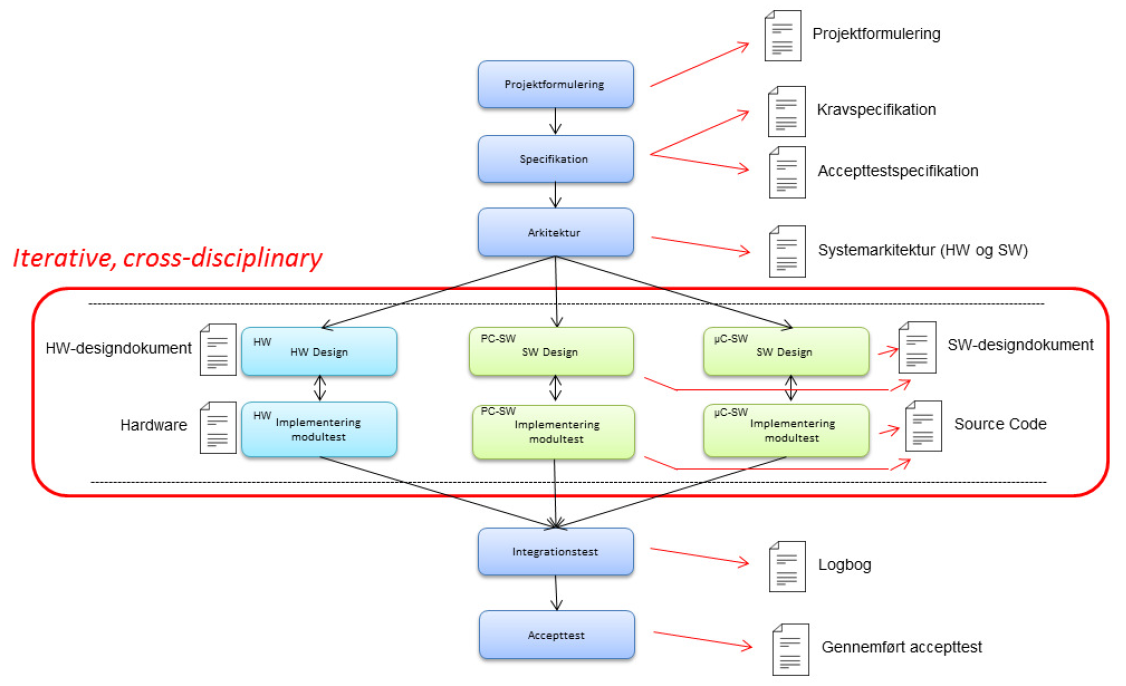
\includegraphics[width=\linewidth]
{Figure/asemodel}}
\caption{ASE-modellen udviklet af Aarhus Ingeniørskole, som bachelorprojektet tager udgangspunkt i.}
\label{asemodel}
\end{figure}



Da bachelorprojektet kræver yderligere test og undersøgelser vil denne ASE-model blive modificeret. Der er tilføjet en ekstra fase, analysefasen. Hvilket resulterer i en anden ASE-model til bachelorprojektet, som kan ses i figur \ref{procesVoresASE}.


\begin{figure}[H] 
\centering
{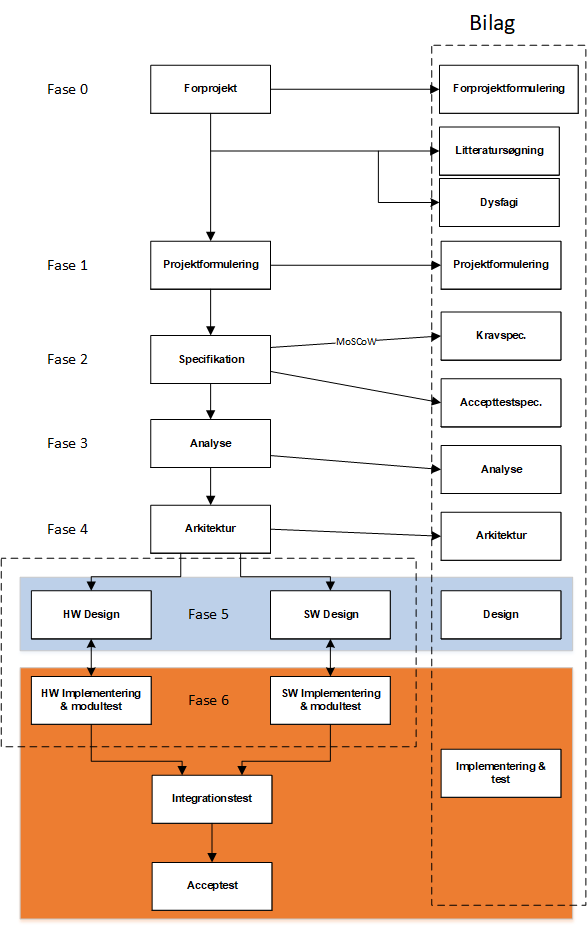
\includegraphics[width=10cm]
{Figure/procesVoresASE}}
\caption{Bachelor projektet med udgangspunkt i ASE-modellen.}
\label{procesVoresASE}
\end{figure}

Bachelorprojektets udvikling blev gennemført i faserne 0 til 6. Faserne er struktureret efter V-modellen\cite{IngeniorhojskolenAarhusUniversiteta}, for at udvikle et veldokumenteret bachelorprojekt. Fase nul bestod i et forprojekt, hvor der blev udarbejdet en projektformulering på baggrund af en udleveret projektbeskrivelse og i samarbejde med vejleder. Her blev der udarbejdet udkast til kravspecifikation (MoSCoW analyse) og projektplan. Disse kan ses i \textit{"bilag 10 - Forprojekt"}. Fase et bestod i at finde videnskabelige litteratur om emnet dysfagi og udvikling af en måler til at detektere synk. Søgeprotokol kan ses i \textit{"bilag 11 - Søgeprotokol"} Dette resulteret i en ny projektformulering.

Ved fase to var nu muligt at opdatere MoSCoW kravene fra forprojektet med den nye viden. Dette resulteret i dokumenterne kravspecifikation og acceptestspecifikation. Kan læses i \textit{"bilag 1 - Kravspecifikation"} og \textit{"bilag 2 - Acceptestspecifikation"}

Den tredje fase begyndte med den nye viden og de nye krav skulle der foretages en analyse. Første del af analysen bestod af at realisere og teste det udleveret kredsløb fra artiklen. Der blev derudover bl.a. undersøgt muligheden for anvendelse af A/D-konverter. Test og undersøgelserne blev til dokumentet Analyse, hvilket kan ses i \textit{"bilag 3 - Analyse"}.

Den fjerde fase blev arkitekturen til software og hardware udført, på baggrund af analysen. Det var nu besluttet hvilke blokke synkerefleksmonitor skulle bestå af. Arkitekturen kan læses i \textit{"bilag 4 - Arkitektur"}

I den femte iterative design fase, blev software og hardware designet. Detaljerne kan læses i \textit{"bilag 5 - Design"}

Til sidst i den sjette fase blev software og hardware implementeret, modultestet og samlet til en integrationstest. Til slut blev acceptest udført. Denne fase er samlet i \textit{"bilag 6 - Implementering \& Test"}.



\begin{figure}[H] 
\centering
{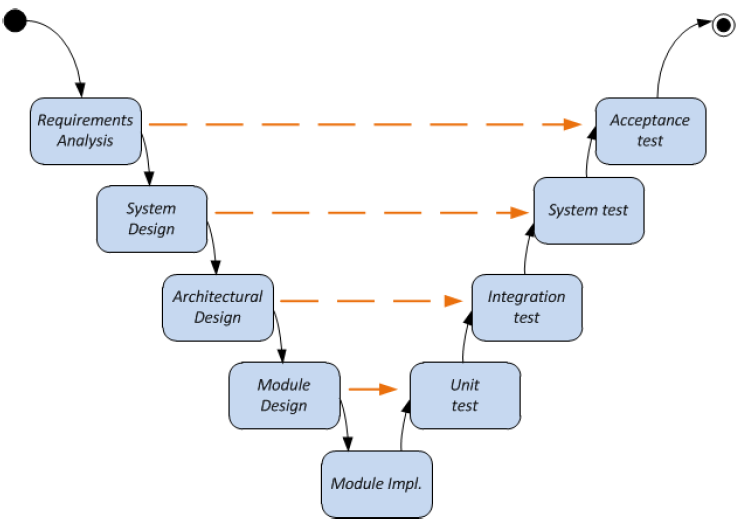
\includegraphics[width=12cm]
{Figure/vmodel}}
\caption{Bachelor projektet med udgangspunkt i ASE-modellen.}
\label{vmodel}
\end{figure}



  
 %\textbf{Forprojekt}\\

%Dette bachelorprojekt udspringer fra et forprojekt af selv samme bachelorgruppe. I forprojektet blev der arbejdet på et udkast til en kravspecifikation og en projektplan. Kravspecifikationen blev udarbejdet vha. en MoSCoW analyse. Denne gjorde det muligt at dele kravene op i en prioriteret rækkefølge.  Projektplanen blev udarbejdet efter ASE-modellen og dens rækkefølge i hvordan et projekt forløber. 
%
%
%Efter udvælgelsen af projektet Synkerefleksmonitor er der blevet lavet et forprojekt. På baggrund af opgavebeskrivelsen blev der lavet et udkast til kravspecifikationen. Her blev der anvendt MoSCoW metoden. Metoden resulteret i hvilke krav vi skulle have løst i prioteret rækkefølge i bachelorprojekt. 
% 
% 
% 
% 
% 
%  men også dem som vi måske ville kunne nå afhængig af tid og kompetencer og til slut dem vi ikke ville kunne lave, men kunne bruges til en fremtid og perspektivering af en videreudvikling af systemet. Revision historikken af MoSCoW analysen kan ses i BilagXX. Fra første udkast til den endelige version med ændringer undervejs. Den endelig Moscow analyse vil være en del af den endelige kravspecifikation. Efter MoSCow analysen var det nu muligt at lave en use case og et udkast til designsammensætningen af software og hardware, da vi kendte behovet igennem opgavebeskrivelsen. Læs første udkast af MosCow, use case, design af software og hardware (diagram) i BilagXX - forprojekt synkerefleksmonitor. 
% 
%Dernæst blev der udarbejdet et udkast til projektplan, hvor der blev overvejet hvilke eksperimenter og teknologier projektet ville anvende igennem hele processen. Dette udkast indeholder alt fra at ex. bygge bioimdedans på fumlebræt, indsamle synkefrekvenser til brug af Latex til rapportskrivning og google drive til dokument håndtering.
%
%Skabeloner til mødeindkaldelser og møderefarat blev også udarbejdet og kan ses i bilagXX.
% 
%Vores bachelorprojekt er en videreførelse af et tideligere bachelorprojekt. Dette omhandlede at undersøge de forskellige teknologier til at måle synkefrekvensen. Så dette projekt er blevet gennemgået for at finde inspiration, erfaringer og mulige referancer herfra. Der blev også søgt efter videnskabelige artikler for at danne et overblik over muligheden for at målesynkefrekvensen. Udover den udleveret videnskabelige artikel fra opgavebeskrivelsen blev der fundet yderligere videnskabelige artikler. Se denne proces i Bilag - søgning af videnskabelige artikler. Der blev samtidtig fundet litteratur i form af undervisningsbøger igennem de forskellige semestre. (SE referance listen?)
% 
%Samtidig med det overstående arbejde, blev der udarbejdet en samarbejdsaftale i samarbejde med vejleder. Aftalen omhandler forventet arbejdsted og tid, roller, gruppens forventninger m.m. Den blev underskrevet og kan ses i Bilag XX - Samarbejdsaftale. Se første udkast af samarbejdsaftalen i Bilag XX - forprojekt Synkerefleksmonitor.
%
%Der blev udarbejdet en overordnet tidsplan for hele bachelorprojektet. Opbygning er efter ASE-modellen og der er derfor muligt at se hvilke områder man skal arbejde i, men samtidig en mulighed for at ændre tidsplanen bachelorprojektet skrider frem. Der blev valgt Teamgantt som er en online portal med et gantt skema som alle gruppens medlemmer har afgang til. Læs nærmere om brugen af TeamGantt i Bilag - Værktøjer. Revision af tidsplan kan ses i Bilag - Tidsplan. 
% 
%Endelig kunne vi lave en konklusion på arbejdet med forprojektet. Hvor vi konkluderet blandt andet at arbejdet med MoSCow analysen har givet en større forståelse og overblik for hvilke krav der er stillet til systemet. Forprojekt gav gruppen et billede og overblik over hvordan forløbet ville nogenlunde se ud og hvilke opgaver og krav gruppen havde stillet sig selv. 



 


\chapter{Projektledelse}
I dette bachelor projekt var der valgt ikke at have en projektleder. Der var i stedet valgt en ligefordelt og kollektiv ledelse. Det har gjort at hele gruppen har skulle have overblik i hele projektet. Samtidig har det været med til at alle i gruppen kender målet og retningen og der er tydelige kommunikation og opfølgninger med faste møder og scrum møder hver dag hvor alle deltager i gruppen. Hvilket har resulteret i at eventuelle forhindringer bliver adresseret og løst undervejs. Den fælles ledelsesstil har gjort at alle deltagerne er engageret og hele tiden kender målet og er klar til at ændre sådan, at målet opnåes på den bedste mulige måde. Da der er mange praktiske opgaver i bachelorprojekt, er der lavet rollefordeling og ansvarsområder igennem hele projektet. De specifikke roller og ansvarsområder kan ses i BilagXX - Samarbejdsaftale.



\chapter{Arbejdsfordeling}
Arbejdesbyrden var ligeligt fordelt i mellem gruppemedlemmerne. Efter interesse og kompetance var det muligt at byde ind på de områder man fandt interssant. Hvor den generelle rapportskrivning af afsnit blev tildelt efter hvem der havde tid og hvad der var bedst for bachelorprojektet. Administrationen  af opgaver blev oprettet og styret fra online portalen Pivotal Tracker. Her blev der i fællesskab oprettet opgaver efter pointsystem om hvor vigtig opgaven var. nu var det så muligt at tage opgaver og udføre de, indenfor for et sprint på en uge. Efter en uge ville man kunne få et overblik over afsluttet opgave i det pågældende sprint. En nærmere beskrivelse og brugen af Pivotal Tracker findes i BilagXX - Værktøjer. 





\chapter{Planlægning}
I den overordnet planlægning blev der bruget online portalen Teamgantt. Her blev der oprettet en kalender over hele forløbet delt op i forskellige områder fra ASE-modellen. Denne kalender havde hele gruppen adgang til og mulighed for at rette løbende gennem hele projektet. Gruppens brugen af Teamgantt og indstillinger kan læses nærmere i BilagXX - værktøjer. For at opreteholde en historik over tidsplanen blev der oprettet en versions historik af tidsplanen, denne kan ses i BilagXX - tidsplan. 

Det daglige arbejde blev nedskrevet i logbogen ved dagens slutning. Logbogen blev også brugt til at notere beslutninger, ændringer og større arbejde ifm. projektet. For at læse den komplette logbog se BilagXX - Logbog.




\chapter{Projektadministration}
Rapporten og bilag er skrevet i Overleaf i tekstsproget Latex. Hvor alle afsnit er delt op i selvstændige .tex filer. Disse afsnit er delt op i en rapport og bilags mappe. Figurer brugt i projektet har også en selvstændig mappe. Møder, referater og logbog er også skrevet i Overleaf og bliver oprettet som selvstændige PDF filer. Tidsplan og opgaver er oprettet og ligger i selvstændige online værktøjerne: Teamgantt og Pivotal Tracker.    


\chapter{Møder}
\section{Interne møder i gruppen}
For at opretholde overblikket og en fast struktur i projektet var der faste møder i gruppen. Hver morgen startet med scrum møde, hvor hvert gruppe medlem fremførte igangværende opgaver og problematikker. Fredagsmødet blev holdt for at kigge tilbage på ugen og det afsluttede sprint. 

\section{Vejledermøder}
Der blev afholdt vejledermøde en gang om ugen. Disse blev brugt til at afstemme fremskridt og opståede spørgsmål i løbet af projektet.

\section{Eksternemøder}
For at udvikle et relevant slutprodukt, blev slutbrugeren løbende inddraget med møder på Hammel Neuro Center med mulighed for feedback og efterfølgende justring af produktets udvikling og mål af gruppen på bag grund af disse. 


\chapter{Konflikthåndtering}
Ved konflikter og samarbejdsproblemer løste parterne problemerne indbyrdes. Ved evt. større konflikter og manglende bidragelse til projektarbejdet inddrages projektvejleder til at hjælpe med den pågældende konflikt. 

\bibliography{library}




































\section*{Tekniske udviklingsværktøjer}
\begin{itemize}
\item ASE-modellen
\item V-modellen
\item SysML
\item UML
\item applikationsmodel
\item domænemodel
\item use case
\item Visio
\item Matlab
\item Overleaf
\item Pivotal tracker
\item Mendeley
\end{itemize}






\section*{Procesværktøjer}
\begin{itemize}
\item TeamGantt
\item Pivotal Tracker
\item samarbejdsaftaler
\item Arbejdsfordeling
\item Planlægning
\item Møder
\item Projektledelse
\item Projektsadministation
\item Google drive
\item Facebook
\item Onenote
\item GradePro
\item 

\end{itemize}





\cite{Aroom2009}

\end{document}



